\documentclass[UTF8,11pt,a4paper]{ctexart}
\usepackage[margin=2.05cm]{geometry}
\usepackage{amsmath,amssymb,bm,booktabs,longtable,array,graphicx,xcolor,hyperref,float,caption,subcaption}
\usepackage{tikz}
\usetikzlibrary{arrows.meta,positioning,shapes.geometric,fit}
\hypersetup{colorlinks=true,linkcolor=blue!55!black,urlcolor=blue!55!black,citecolor=blue!55!black}
\setlength{\parindent}{2em}
\setlength{\parskip}{0.30em}
\definecolor{deep}{RGB}{30,58,95}
\definecolor{good}{RGB}{23,112,70}
\definecolor{warn}{RGB}{178,91,20}
\definecolor{soft}{RGB}{240,244,249}
\newcommand{\mat}[1]{\bm{#1}}
\newcommand{\vect}[1]{\bm{#1}}
\newcommand{\key}[1]{\textcolor{deep}{\textbf{#1}}}
\newcommand{\code}[1]{\texttt{#1}}
\newcommand{\R}{\mathbb{R}}
\newcommand{\C}{\mathbb{C}}
\graphicspath{{../../}}

\title{\textbf{面向高频变压器逐匝耦合参数辨识的图神经网络方法}\
\large 网络结构、物理解码、基线比较与现阶段证据的完整技术报告}
\author{基于 EXP15--EXP25 代码、结果文件与阶段报告整理}
\date{2026年9月18日}

\begin{document}
\maketitle

\begin{abstract}
本报告只讨论逐匝图神经网络（graph neural network, GNN）及其参数辨识链路，不纳入早期集中参数、传递零点或端口级 $C_{ps}$ 辨识实验。当前项目把高频变压器表示为包含导电连接、电容耦合和磁耦合的逐匝多关系图，并以可微矩阵/Kron 求解器作为物理解码器。实验链依次验证了四项能力：FALCON 风格正向图代理能否学习参数图到响应的映射；关系分型和 edge-centric 消息能否改善内部量预测；网络能否选择应保留的耦合边；以及在 COMSOL 教师和 DAB 多窗口观测下，网络能否反演低维物理合法参数并更新耦合边。现有证据表明，edge-centric 表示对端口和内部电压任务有小幅稳定收益，可学习门控能在固定预算下接近任务 oracle，COMSOL 教师驱动的五维反演闭环已经跑通，且测量条件化边更新可将端口响应误差由 2.381\% 降至 1.618\%。同时，实验也给出了明确边界：当前 GNN 尚未在模型失配下超过纯物理反演，逐条互感变化定位低于随机基线，56 维边更新在现有两端口观测下只有约 3 个强可辨识组合方向。因此，现阶段最可信的主方法不是“端口测量直接恢复全部逐匝矩阵”，而是“静态耦合结构先验 + Fisher 可辨识低维模态 + 测量条件化 GNN + 精确物理解码”。
\end{abstract}

\tableofcontents
\newpage

\section{报告范围与核心结论}

\subsection{本报告包含什么}
本文覆盖 EXP15--EXP25 中与 GNN 直接相关的内容：
\begin{enumerate}
  \item 逐匝图数据契约和可微物理矩阵求解器；
  \item FALCON 风格同质 GNN、HFT 分型 GNN 与 edge-centric 异构 GNN；
  \item absolute 与 residual 正向代理任务；
  \item 可学习跨绕组电容边门控；
  \item COMSOL 教师驱动的五维物理合法参数反演；
  \item 模型失配下的 GNN、纯物理和混合反演比较；
  \item 静态耦合边选择与测量条件化的动态边更新；
  \item Fisher/SVD 可辨识图模态及 DAB PWM 多窗口观测边界。
\end{enumerate}

本文不把早期端口集中参数实验重新写入，也不把端口导纳重构本身作为主要贡献。端口量在这里仅承担两项作用：作为 GNN 的可测输入，以及作为物理解码后的外部一致性验证量。

\subsection{一句话论点}
在逐匝耦合参数数量远大于端口独立观测维数的条件下，本项目已经证明图网络可以学习\emph{耦合结构重要性和低维参数更新}，但尚不能从两端口自然 PWM 数据唯一恢复全部 $C_{ij}$ 和 $M_{ij}$；可靠路线必须把 GNN 输出限制在物理合法且 Fisher 可辨识的低维图参数空间，并由矩阵求解器完成最终响应验证。

\subsection{术语与符号约定}
\begin{longtable}{p{0.23\linewidth}p{0.68\linewidth}}
\toprule
术语 & 本报告中的固定含义\\
\midrule
逐匝图 & 每个导体匝或等效导体段作为图实体，边表示电气连续性、电容耦合或磁耦合\\
正向代理 & 已知图结构和参数，预测端口响应、内部电压或耦合电流\\
参数反演 & 已知测量响应，估计低维物理参数或边更新量\\
边选择 & 在给定预算下决定哪些候选 $C_{ij}$ 或 $M_{ij}$ 应保留\\
边更新 & 依据运行测量估计边参数相对正常模型的变化\\
物理解码 & 将网络输出重新组装为 $\mat R,\mat L,\mat C$，再调用可微矩阵/Kron 求解器\\
FALCON baseline & 借鉴 FALCON 的同质消息传递和图级读出思想，由本项目重新实现的 HFT 基线，而非原仓库完整复现\\
\bottomrule
\end{longtable}

\section{研究任务：GNN究竟辨识什么}

\subsection{高维逐边问题}
设原、副边总计 $N$ 个导体匝。候选无向匝对数为
\begin{equation}
N_e=\frac{N(N-1)}{2}.
\end{equation}
如果每个匝对同时包含互电容和互感，待更新维数可达到 $2N_e$。以当前 $4+4$ 匝模型为例，$N=8$，已有 $28$ 个无向匝对和 $56$ 个 $C/M$ 边更新自由度。若直接令
\begin{equation}
\vect z=[\Delta\log C_{12},\ldots,\Delta\log C_{N-1,N},
\Delta\log M_{12},\ldots,\Delta\log M_{N-1,N}]^{\mathsf T},
\end{equation}
从两端口数据自由恢复 $\vect z$，问题在数值上严重病态。

\subsection{当前方法把任务拆成三层}
\begin{figure}[H]
\centering
\resizebox{\linewidth}{!}{%
\begin{tikzpicture}[node distance=7mm and 9mm,>=Latex,
box/.style={draw=deep,rounded corners,fill=soft,align=center,minimum height=10mm,text width=4.0cm},
arr/.style={->,thick,deep}]
\node[box] (teacher) {高保真教师\\COMSOL $\mat C_0,\mat L_0$\\或正常状态标定};
\node[box,right=of teacher] (graph) {逐匝多关系图\\节点、候选边、几何属性};
\node[box,right=of graph] (selector) {静态边选择 GNN\\输出重要性分数};
\node[box,below=of graph] (measurement) {DAB 多窗口测量\\$v_1,i_1,v_2,i_2$};
\node[box,right=of measurement] (updater) {测量条件化 GNN\\输出低维模态或边更新};
\node[box,right=of updater] (physics) {物理解码器\\组装 $\mat R,\mat L,\mat C$\\Kron 求解};
\draw[arr] (teacher)--(graph);
\draw[arr] (graph)--(selector);
\draw[arr] (graph)--(updater);
\draw[arr] (measurement)--(updater);
\draw[arr] (selector)--(physics);
\draw[arr] (updater)--(physics);
\end{tikzpicture}%
}
\caption{逐匝 GNN 参数辨识的三层结构。GNN不直接取代电路求解器，而是决定结构和参数更新。}
\end{figure}

三层任务分别是：
\begin{enumerate}
  \item \textbf{静态结构：}在正常/标称模型中确定哪些耦合边重要；
  \item \textbf{动态更新：}由运行测量估计哪些耦合组合发生变化；
  \item \textbf{状态恢复：}用物理解码后的矩阵计算端口响应、内部电压和位移电流。
\end{enumerate}

\section{逐匝物理图与可微矩阵求解器}

\subsection{电位节点与导体支路}
严格的电路模型需要区分电位节点与导体段。设非参考电位向量为 $\vect v\in\C^{N_v}$，导体支路电流为 $\vect i_b\in\C^{N_b}$，支路--节点关联矩阵为 $\mat A\in\R^{N_v\times N_b}$。串联阻抗矩阵为
\begin{equation}
\mat Z_b(\omega)=\mat R(\omega)+j\omega\mat L(\omega),
\end{equation}
其中 $\mat L$ 的对角元为自感，非对角元包含互感。支路关系和节点 KCL 为
\begin{equation}
\mat A^{\mathsf T}\vect v=\mat Z_b\vect i_b,
\qquad
\vect i=\mat A\vect i_b+(\mat G+j\omega\mat C)\vect v.
\end{equation}
消去 $\vect i_b$ 后得到节点导纳
\begin{equation}
\boxed{\mat Y_n(\omega)=\mat A\mat Z_b^{-1}(\omega)\mat A^{\mathsf T}+\mat G+j\omega\mat C.}
\label{eq:Yn}
\end{equation}
实现中使用线性方程求解而非显式矩阵求逆，以保持数值稳定和自动微分图。

\subsection{Kron消元和内部状态恢复}
把节点分成外部端口 $p$ 和内部节点 $q$：
\begin{equation}
\begin{bmatrix}\vect i_p\\\vect 0\end{bmatrix}=
\begin{bmatrix}\mat Y_{pp}&\mat Y_{pq}\\\mat Y_{qp}&\mat Y_{qq}\end{bmatrix}
\begin{bmatrix}\vect v_p\\\vect v_q\end{bmatrix}.
\end{equation}
则
\begin{equation}
\vect v_q=-\mat Y_{qq}^{-1}\mat Y_{qp}\vect v_p,
\end{equation}
\begin{equation}
\boxed{\mat Y_{port}=\mat Y_{pp}-\mat Y_{pq}\mat Y_{qq}^{-1}\mat Y_{qp}.}
\label{eq:kron}
\end{equation}
式\eqref{eq:kron}同时提供端口响应与内部电压。对跨绕组电容边 $(i,j)$，第 $h$ 个谐波位移电流为
\begin{equation}
I_{ij,h}=j2\pi f_h C_{ij}(V_{i,h}-V_{j,h}),
\qquad
I_{ij,\mathrm{rms}}=\sqrt{\sum_h|I_{ij,h}|^2}.
\end{equation}

\subsection{物理合法性}
物理解码必须满足：
\begin{align}
&\mat L=\mat L^{\mathsf T},\quad \mat L\succ0,\\
&\mat C=\mat C^{\mathsf T},\quad \mat C\succeq0,\\
&C_{ij}\le0\;(i\ne j)\quad\text{(Maxwell/拉普拉斯盖章约定)},\\
&\mat Y_{port}=\mat Y_{port}^{\mathsf T}\quad\text{(互易条件)},\\
&\Re\{\mat Y_{port}\}\succeq0\quad\text{(无源条件)}.
\end{align}
EXP15 已验证 4+4 和 8+8 模型的新旧端口矩阵相对误差分别为 $2.06\times10^{-15}$ 和 $4.95\times10^{-15}$，内部 KCL 残差约 $2.0\times10^{-14}$ A。这证明物理教师实现自洽，但不代表其演示参数来自真实样机。

\begin{figure}[H]
\centering
\begin{tikzpicture}[scale=.88,transform shape,>=Latex,
tn/.style={circle,draw=deep,fill=soft,minimum size=7mm,font=\small},
se/.style={thick,deep}, ce/.style={thin,orange!80!black,bend left=14},
me/.style={dashed,good,bend right=18}]
\foreach \i in {1,...,8}{\node[tn] (p\i) at (\i*1.05,1.35) {$P_{\i}$};
\node[tn] (s\i) at (\i*1.05,-1.35) {$S_{\i}$};}
\foreach \i [evaluate=\i as \j using int(\i+1)] in {1,...,7}{
\draw[se] (p\i)--(p\j); \draw[se] (s\i)--(s\j);}
\foreach \i in {1,...,8}{\draw[ce] (p\i) to (s\i);}
\draw[me] (p1) to (s8); \draw[me] (p8) to (s1);
\node[align=left,anchor=west] at (9.7,1.2) {实线：串联边\\橙线：跨绕组电容\\绿虚线：非局部磁耦合};
\end{tikzpicture}
\caption{8+8 匝多关系图结构示意。图用于表达多类型耦合，物理响应仍由矩阵方程计算。}
\end{figure}

\section{GNN输入、消息传递与输出头}

\subsection{节点和边特征}
当前网络使用匝级节点。典型节点特征包括绕组身份、归一化轴向位置、端口标记、局部 $R/L$ 信息以及 DAB 工况。边分为四类：
\begin{longtable}{p{0.18\linewidth}p{0.28\linewidth}p{0.45\linewidth}}
\toprule
边类型 & 参数 & 物理作用\\
\midrule
series & $R_i,L_i$、方向、距离 & 同一绕组的电气连续性和纵向传播\\
local-cap & 相邻匝、层间、对地电容 & 局部电场储能与电压梯度\\
cross-cap & $C_{ij}^{ps}$、重叠、距离 & 跨隔离屏障位移电流和共模源项\\
magnetic & $M_{ij}$、符号、公共磁通关系 & 主磁通与漏磁的局部/非局部耦合\\
\bottomrule
\end{longtable}

\subsection{FALCON风格同质基线}
同质基线把所有关系合并：
\begin{equation}
\vect h_i^{(\ell+1)}=\mathrm{LN}\!\left(\vect h_i^{(\ell)}+
\mat W_s\vect h_i^{(\ell)}+
\sum_{j\in\mathcal N(i)}\widetilde a_{ij}\mat W_m\vect h_j^{(\ell)}\right).
\end{equation}
其优点是参数少、实现稳定；缺点是串联边、电容边和磁耦合边在消息函数中没有不同的物理语义。该模型只借鉴 FALCON 的 edge-aware 图代理思想和图级读出框架，是本项目自建 baseline。

\subsection{HFT typed GNN}
分型网络为每种关系建立独立变换：
\begin{equation}
\vect m_i^{(\ell)}=\sum_{r\in\mathcal R}\sum_{j\in\mathcal N_r(i)}
\widetilde a_{ij}^{(r)}\mat W_r^{(\ell)}\vect h_j^{(\ell)}.
\end{equation}
它能区分边类型，但连续边属性通常只作为权重，不能充分表达 $C_{ij}$、$M_{ij}$、距离和方向的联合效应。

\subsection{Edge-centric异构GNN}
edge-centric 模型对每类边使用独立边消息网络：
\begin{equation}
\vect m_{ij}^{(r)}=\mathrm{MLP}_r\left([\vect h_i,\vect h_j,\vect e_{ij}]\right),
\quad
\vect h_i^{(\ell+1)}=\mathrm{LN}\left(\vect h_i^{(\ell)}+
\sum_r\sum_{j\in\mathcal N_r(i)}\vect m_{ij}^{(r)}\right).
\end{equation}
这使边参数成为消息内容，而不仅是邻接关系。EXP18 使用隐藏维度 56、3 层残差消息传递；EXP21 的 COMSOL 反演网络约 73,925 个参数；EXP23 的边选择与更新网络约 34,206 个参数。

\subsection{三类输出头}
\begin{enumerate}
  \item \textbf{图级头：}读出 $Y_{11},Y_{22},Y_{12}$ 等端口复响应；
  \item \textbf{节点头：}输出逐匝内部电压或局部状态；
  \item \textbf{边头：}输出位移电流、边重要性分数、边变化概率或有界 $\Delta\log C_{ij},\Delta\log M_{ij}$。
\end{enumerate}
本项目后期的关键变化，是把网络输出从“响应”改成“边结构和参数更新”，再由式\eqref{eq:Yn}--\eqref{eq:kron}完成物理解码。

\section{训练任务的演化}

\subsection{正向absolute与residual任务}
Absolute 模式直接预测完整响应
\begin{equation}
\widehat{\vect y}=f_\phi(\mathcal G,\vect u),
\end{equation}
Residual 模式先计算标称物理响应，再只学习变化
\begin{equation}
\widehat{\vect y}=\vect y_0+\Delta\widehat{\vect y}_{GNN}.
\end{equation}
EXP18 的多任务损失为
\begin{equation}
\mathcal L=\mathcal L_{port}+0.7\mathcal L_{node}+0.5\mathcal L_{edge}
+0.05\mathcal L_{passive}.
\end{equation}
Residual 模式更接近在线变化监测，但它仍是响应预测，不等同于参数辨识。

\subsection{可学习耦合边门控}
EXP19 对每条跨绕组电容候选边输出分数 $s_{ij}$，在固定预算下执行 top-$k$：
\begin{equation}
g_{ij}=\mathrm{TopK}(s_{ij}),\qquad \widetilde C_{ij}=g_{ij}C_{ij}.
\end{equation}
训练使用 straight-through 近似，使正向已经执行硬裁剪，反向仍能传播梯度。最终响应必须由裁剪后的物理矩阵重新计算。

\subsection{低维物理合法参数反演}
EXP21 不自由输出全部边，而输出五个对数修正坐标
\begin{equation}
\vect\theta=[\theta_{IT},\theta_{WW},\theta_{TC},\theta_m,\theta_\ell]^{\mathsf T}.
\end{equation}
前三个控制匝间、跨绕组、对参考导体电容，后两个控制主磁通和漏磁模态：
\begin{equation}
\mat L(\vect\theta)=e^{\theta_m}\lambda_1\vect u_1\vect u_1^{\mathsf T}
+e^{\theta_\ell}\sum_{q=2}^{N}\lambda_q\vect u_q\vect u_q^{\mathsf T}.
\end{equation}
损失为参数监督与物理残差的组合：
\begin{equation}
\mathcal L_{21}=\|\widehat{\vect\theta}-\vect\theta\|_2^2
+0.02\|\mat Y_{port}(\widehat{\vect\theta})-\widehat{\mat Y}_{meas}\|_2^2.
\end{equation}

\subsection{测量条件化逐边更新}
EXP23 令
\begin{equation}
C_{ij}=C_{ij,0}e^{\delta^C_{ij}},\qquad
M_{ij}=M_{ij,0}e^{\delta^M_{ij}},
\end{equation}
网络输入正常图和相对标称的测量创新量
\begin{equation}
\Delta\mat Y_{obs}=\frac{\widehat{\mat Y}_{obs}-\mat Y_0}{|\mat Y_0|+\varepsilon},
\end{equation}
输出静态重要性、变化概率与有界对数修正。电容矩阵重新盖章，电感矩阵对称化并修复正定性，最终用物理求解器复算响应。

\section{数据来源与先验强度}

\subsection{三代教师数据}
\begin{longtable}{p{0.15\linewidth}p{0.29\linewidth}p{0.46\linewidth}}
\toprule
阶段 & 教师来源 & 可支持的结论\\
\midrule
EXP15--19 & 人工透明 $\mat R/\mat L/\mat C$ 与精确矩阵求解器 & 算法结构、物理闭环和率失真趋势；不能证明真实几何精度\\
EXP20--23 & 12 个参数化 4+4 匝 COMSOL 轴对称几何 & COMSOL 教师下的跨几何可行性；不能证明跨磁芯/三维端部/实机泛化\\
未来实机 & 正常状态标定与运行测量 & 验证仿真到实物迁移、测量链路和真实异常可辨识性\\
\bottomrule
\end{longtable}

EXP21 的 12 个 COMSOL 几何由原副边间隙 1.0/1.5/2.0 mm、匝间距 0.15/0.25 mm 和副边轴向错位 0/0.625 mm 组合而成。每个几何通过 8 次端子电荷求解提取 $\mat C$，通过 36 次磁能组合求解提取 $\mat L$。训练/验证/测试按 8/2/2 几何隔离。

\begin{figure}[H]
\centering
\begin{subfigure}{.48\linewidth}\centering
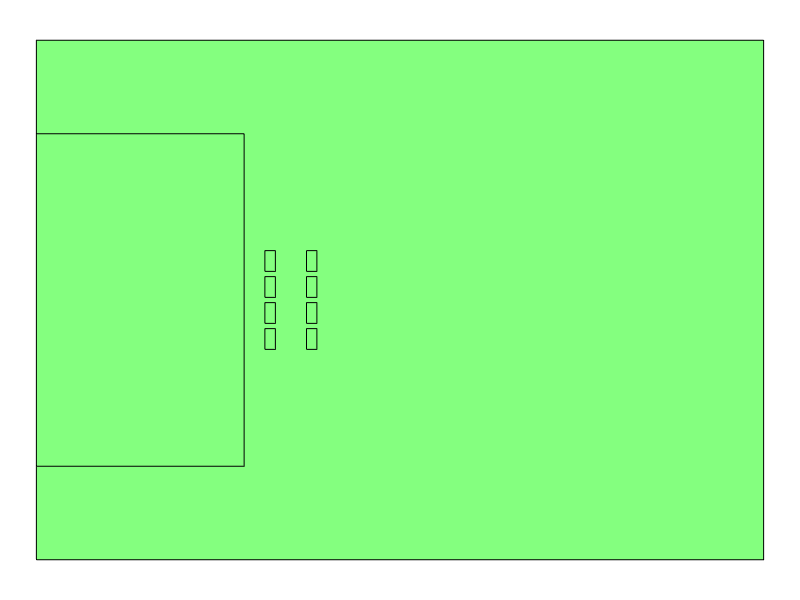
\includegraphics[width=\linewidth]{experiments/experiment20_comsol_turn_matrix_teacher_20260915/figures/convergence/geometry.png}
\caption{4+4 匝轴对称 COMSOL 几何}
\end{subfigure}\hfill
\begin{subfigure}{.48\linewidth}\centering
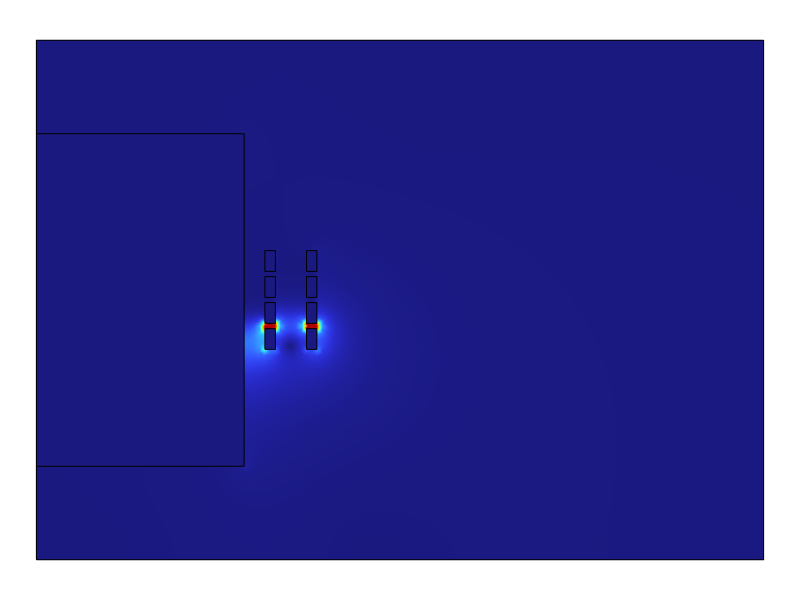
\includegraphics[width=\linewidth]{experiments/experiment20_comsol_turn_matrix_teacher_20260915/figures/convergence/P1_S1_coupled_field.png}
\caption{代表性电磁耦合场分布}
\end{subfigure}
\caption{COMSOL 教师为 GNN 提供逐匝矩阵先验，而不是在线阶段的故障真值。}
\end{figure}

\subsection{先验信息的正确角色}
当前可接受的先验包括正常状态几何、匝连接、材料范围、COMSOL 标称矩阵、离线端口标定和物理合法性。在线算法应辨识相对于正常模型的变化：
\begin{equation}
\mat C(t)=\mat C_0+\sum_{q=1}^{r_C}z_q^C\mat B_q^C,
\qquad
\mat L(t)=\mat L_0+\sum_{q=1}^{r_L}z_q^L\mat B_q^L.
\end{equation}
不能把故障状态的真实逐边矩阵提供给在线网络后再宣称由测量辨识。后续报告应同时给出弱先验、等价先验和强先验三档消融。

\section{基线与公平比较协议}

\subsection{基线分类}
\begin{longtable}{p{0.23\linewidth}p{0.29\linewidth}p{0.38\linewidth}}
\toprule
基线 & 输入/输出 & 回答的问题\\
\midrule
标称模型（zero update） & 正常 $\mat C_0,\mat L_0$，不更新 & 不辨识时能达到什么水平\\
FALCON homogeneous & 同质图 $\rightarrow$ 响应 & 图结构本身是否足够\\
HFT typed & 分型关系图 $\rightarrow$ 响应 & 边类型是否提供增益\\
Edge-centric GNN & 节点+连续边属性 $\rightarrow$ 响应/参数 & 显式边物理是否有效\\
距离/幅值/Fisher门控 & 固定规则 $\rightarrow$ 边子集 & 学习门控是否超越简单规则\\
Oracle门控 & 使用测试样本真实任务重要性 & 给定标签定义下的上限，不是可部署方法\\
纯物理反演 & 测量 $\rightarrow$ 非线性最小二乘 & GNN是否真正增加精度或只增加复杂度\\
GNN直接反演 & 测量+图 $\rightarrow$ 参数 & 无迭代快速估计能力\\
GNN+物理反演 & GNN初值/正则中心+最小二乘 & GNN能否改善收敛、速度或抗失配性\\
随机边选择/定位 & 随机保留或随机猜活跃边 & 边选择和定位是否超过机会水平\\
\bottomrule
\end{longtable}

\subsection{公平性要求}
所有神经网络比较需使用同一数据划分、同一输出任务、相近参数量、相同训练预算和相同物理解码器。参数反演比较必须同时报告：参数误差、端口重构误差、相对于标称模型的增益、运行时间和物理合法率。只比较端口拟合误差会掩盖内部参数错误。

\section{实验结果：正向GNN与耦合结构学习}

\subsection{EXP16：FALCON基线能跑通，但分型网络没有自动获益}
EXP16 中 homogeneous GNN 的归一化响应 MAE 为 0.0521，typed GNN 为 0.0538。后者未胜出，说明仅增加边类型标签并不会自动改善模型；连续边参数、任务监督和消息函数必须配合。

\begin{figure}[H]
\centering
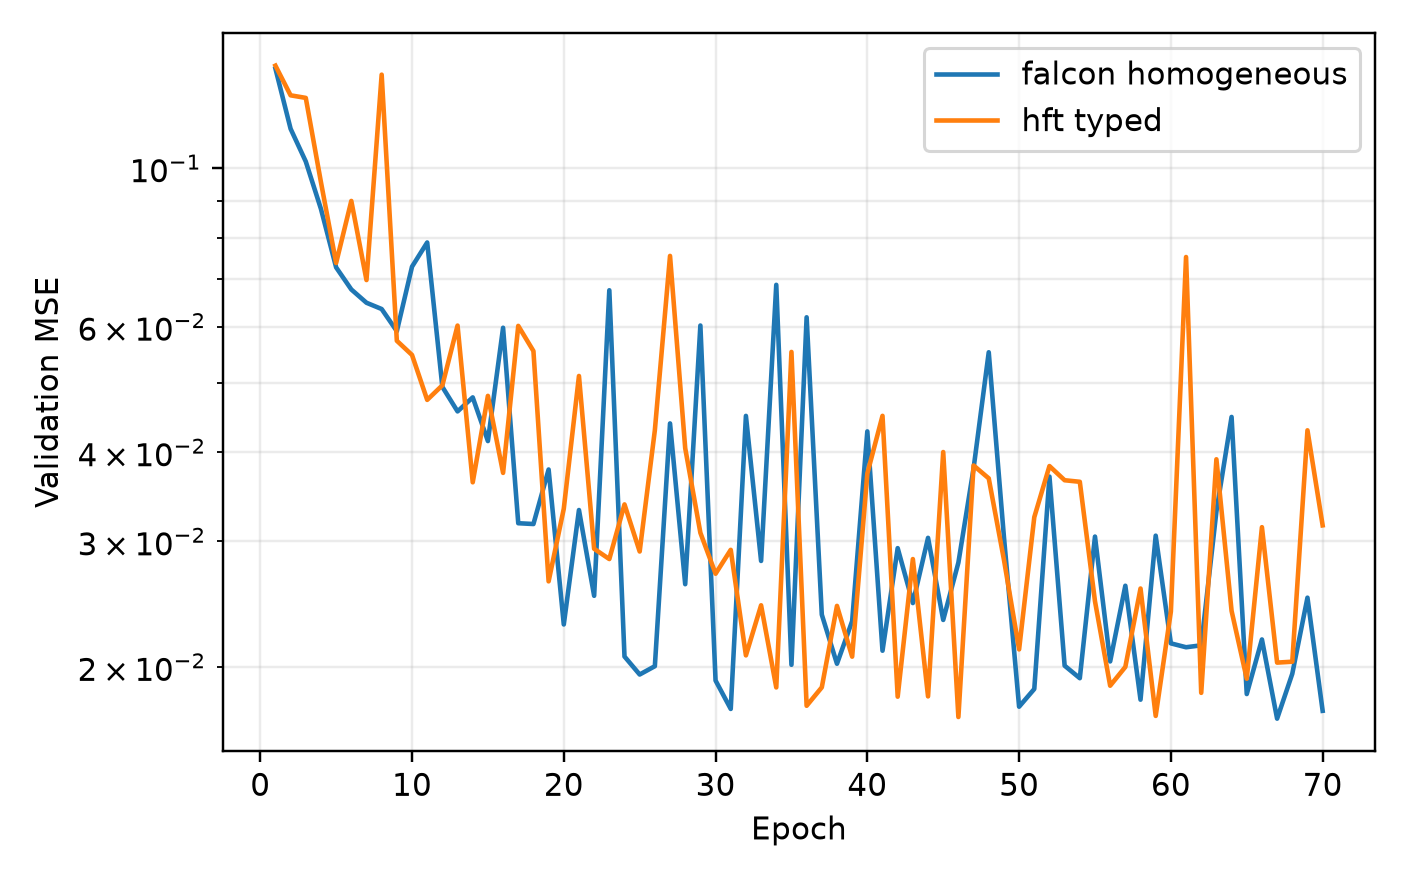
\includegraphics[width=.72\linewidth]{experiments/experiment16_falcon_hft_gnn_20260909/results/training_curves.png}
\caption{EXP16 两类 GNN 的训练/验证曲线。该实验建立了可复现图代理基线。}
\end{figure}

同一实验中的物理反演响应损失达到 $3.02\times10^{-7}$，但八个结构化尺度的平均误差仍为 7.16\%，Jacobian 条件数为 1368.85。这说明低响应损失并不保证参数唯一。

\begin{figure}[H]
\centering
\begin{subfigure}{.48\linewidth}\centering
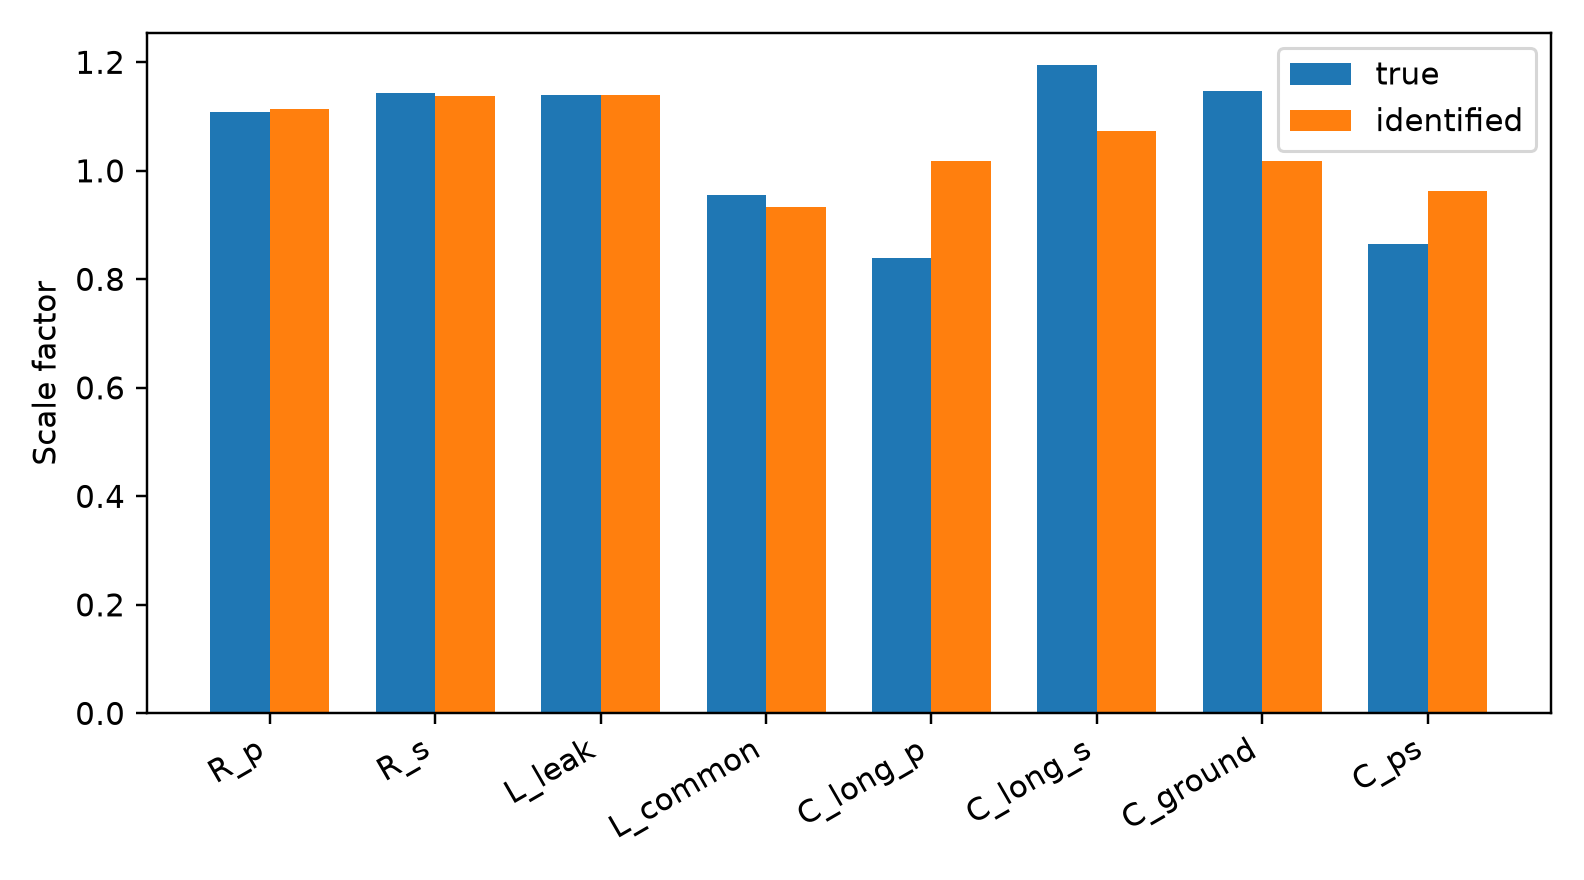
\includegraphics[width=\linewidth]{experiments/experiment16_falcon_hft_gnn_20260909/results/physics_inverse_scales.png}
\caption{参数缩放反演}
\end{subfigure}\hfill
\begin{subfigure}{.48\linewidth}\centering
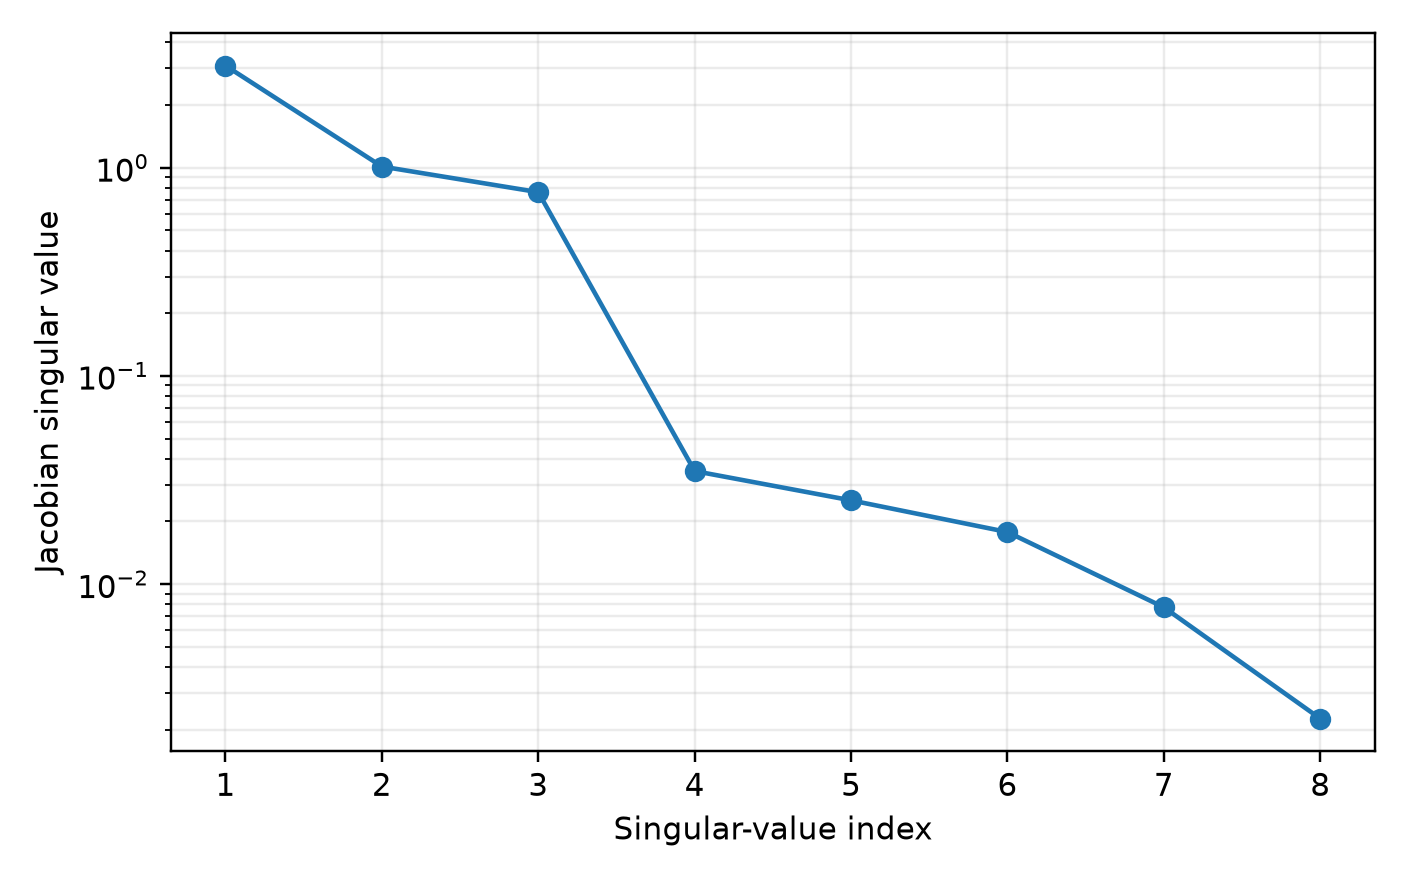
\includegraphics[width=\linewidth]{experiments/experiment16_falcon_hft_gnn_20260909/results/identifiability_spectrum.png}
\caption{灵敏度奇异值谱}
\end{subfigure}
\caption{响应拟合准确与参数恢复准确是两个不同问题。}
\end{figure}

\subsection{EXP18：edge-centric在内部任务上只有小幅优势}
\begin{table}[H]
\centering
\caption{EXP18 residual 测试结果，数值越低越好，峰值命中率越高越好。}
\begin{tabular}{lcccc}
\toprule
模型 & 端口 MAE & 节点 MAE & 边电流 log-MAE & 峰值命中率\\
\midrule
Homogeneous & 0.02845 & 0.004515 & \textbf{0.01211} & 12.08\%\\
Typed & 0.02790 & 0.004328 & 0.01337 & \textbf{13.33\%}\\
Edge-centric & \textbf{0.02707} & \textbf{0.004263} & 0.01230 & 12.50\%\\
\bottomrule
\end{tabular}
\end{table}
Edge-centric 相对 homogeneous 的端口和节点误差改善约 4.84\% 和 5.58\%，但边电流略差。因此可信结论是“显式边属性对部分任务有小幅作用”，而不是“复杂 GNN 已明显优于基线”。

\begin{figure}[H]
\centering
\begin{subfigure}{.48\linewidth}\centering
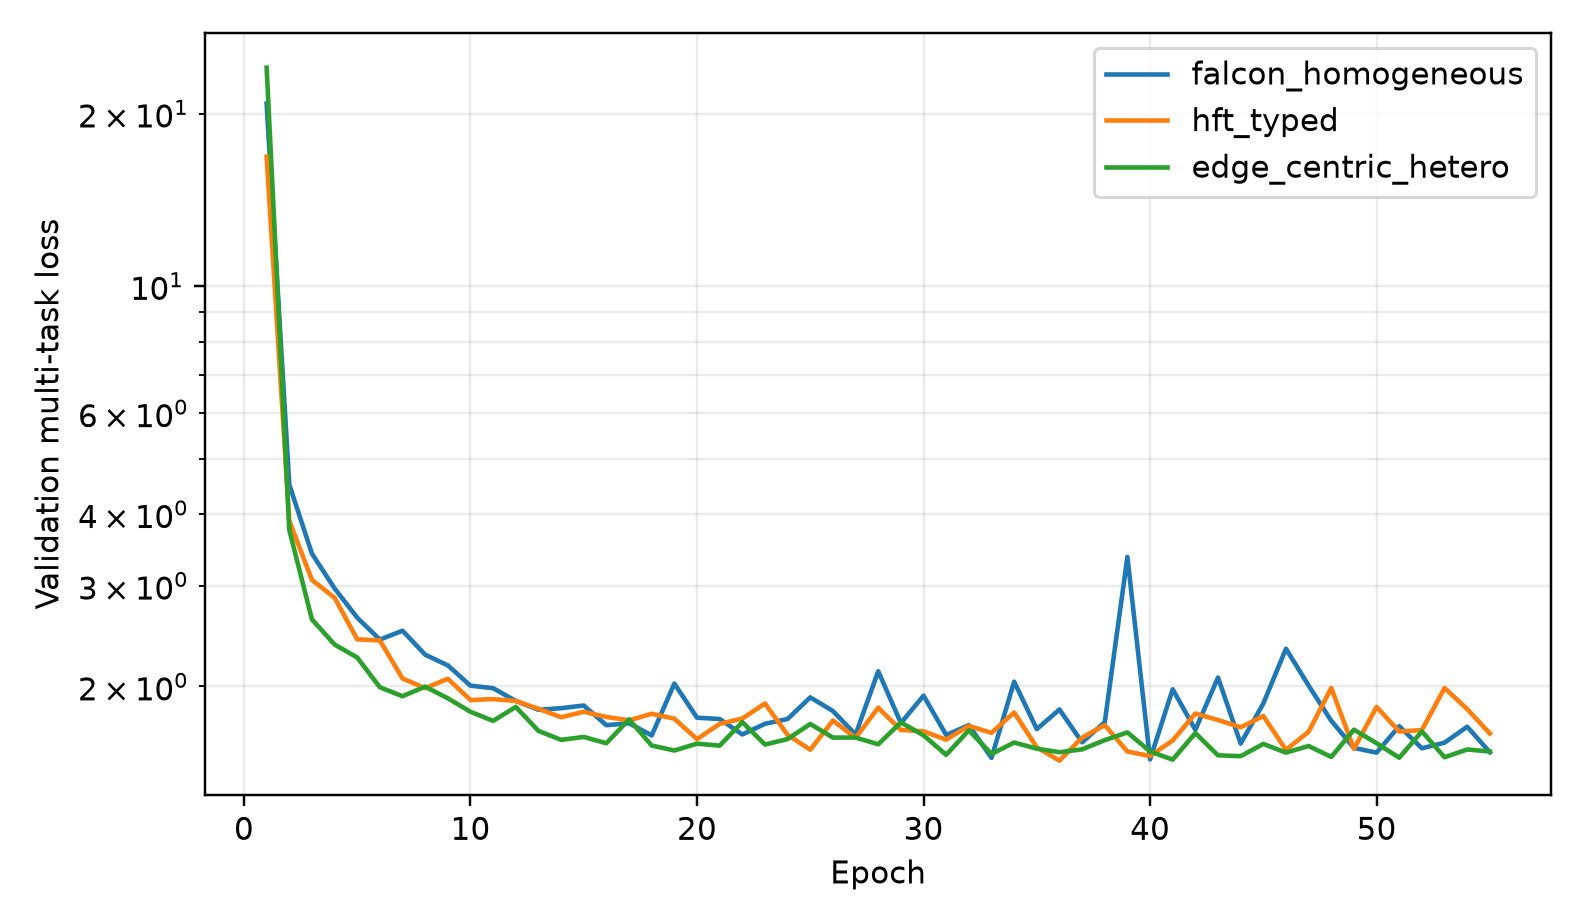
\includegraphics[width=\linewidth]{experiments/experiment18_local_hetero_gnn_20260910/results/residual/training_curves.png}
\caption{Residual训练曲线}
\end{subfigure}\hfill
\begin{subfigure}{.48\linewidth}\centering
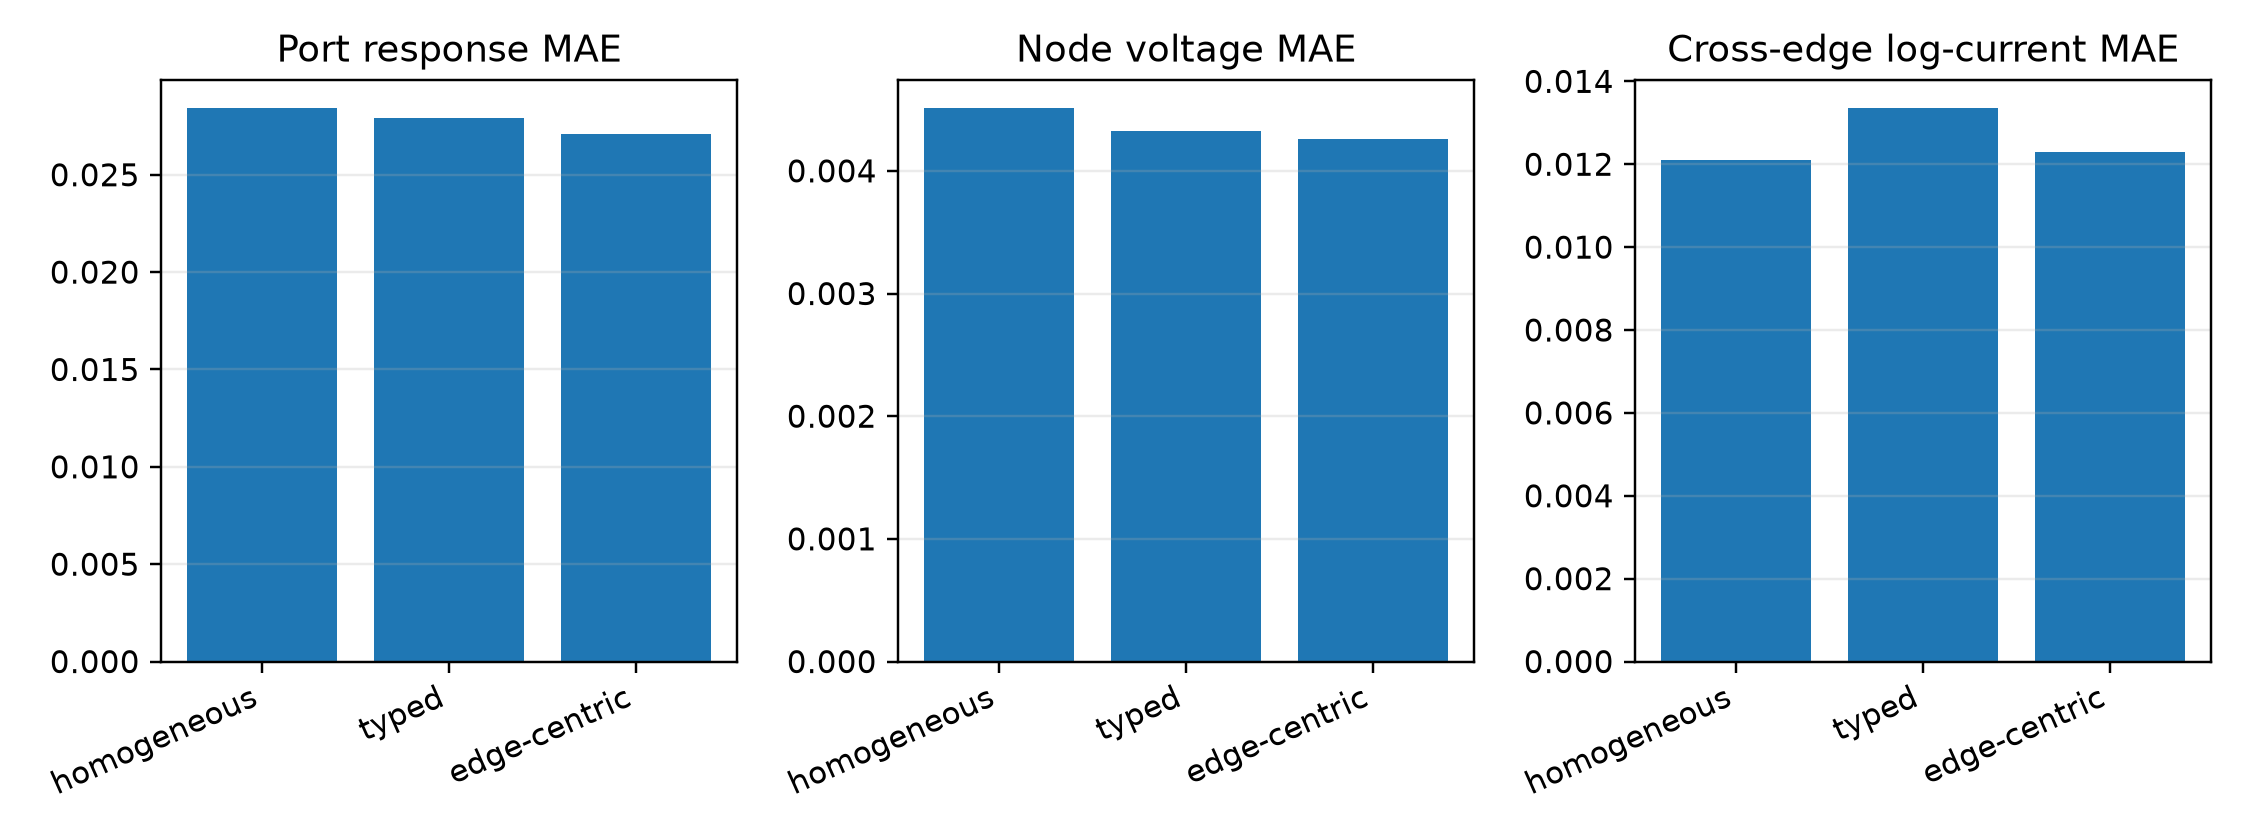
\includegraphics[width=\linewidth]{experiments/experiment18_local_hetero_gnn_20260910/results/residual/test_task_comparison.png}
\caption{三类网络测试对比}
\end{subfigure}
\caption{EXP18 的网络结构比较。}
\end{figure}

Absolute 模式 edge-centric 无源率为 87.33\%，homogeneous 为 76.92\%；软无源惩罚有帮助，但未形成严格保证。Residual 模式峰值位置命中率只有 12--13\%，且随匝数增加显著下降，说明内部局部峰值定位尚未解决。

\subsection{EXP19：网络能选对边，但当前电容图不能激进裁剪}
在相同 40\% 边预算下：
\begin{table}[H]
\centering
\caption{EXP19 跨绕组电容边选择对比。}
\begin{tabular}{lccc}
\toprule
方法 & 端口响应 MAE & 位移电流误差 & 位移电流 p95\\
\midrule
距离 & $2.148\times10^{-6}$ & 35.42\% & 45.97\%\\
电容量级 & $2.048\times10^{-6}$ & 33.71\% & 42.16\%\\
Fisher proxy & $\sim1.3\times10^{-6}$ & $\sim29$--30\% & $\sim35$\%\\
Oracle & $1.344\times10^{-6}$ & 27.98\% & 34.18\%\\
Learned gate & $1.356\times10^{-6}$ & 28.01\% & 34.18\%\\
\bottomrule
\end{tabular}
\end{table}
可学习门控几乎达到 oracle，但 28.01\% 的位移电流误差仍不可接受。率失真扫描显示，若暂以 5\% 为门槛，需要保留约 80\% 的跨绕组电容边。

\begin{figure}[H]
\centering
\begin{subfigure}{.48\linewidth}\centering
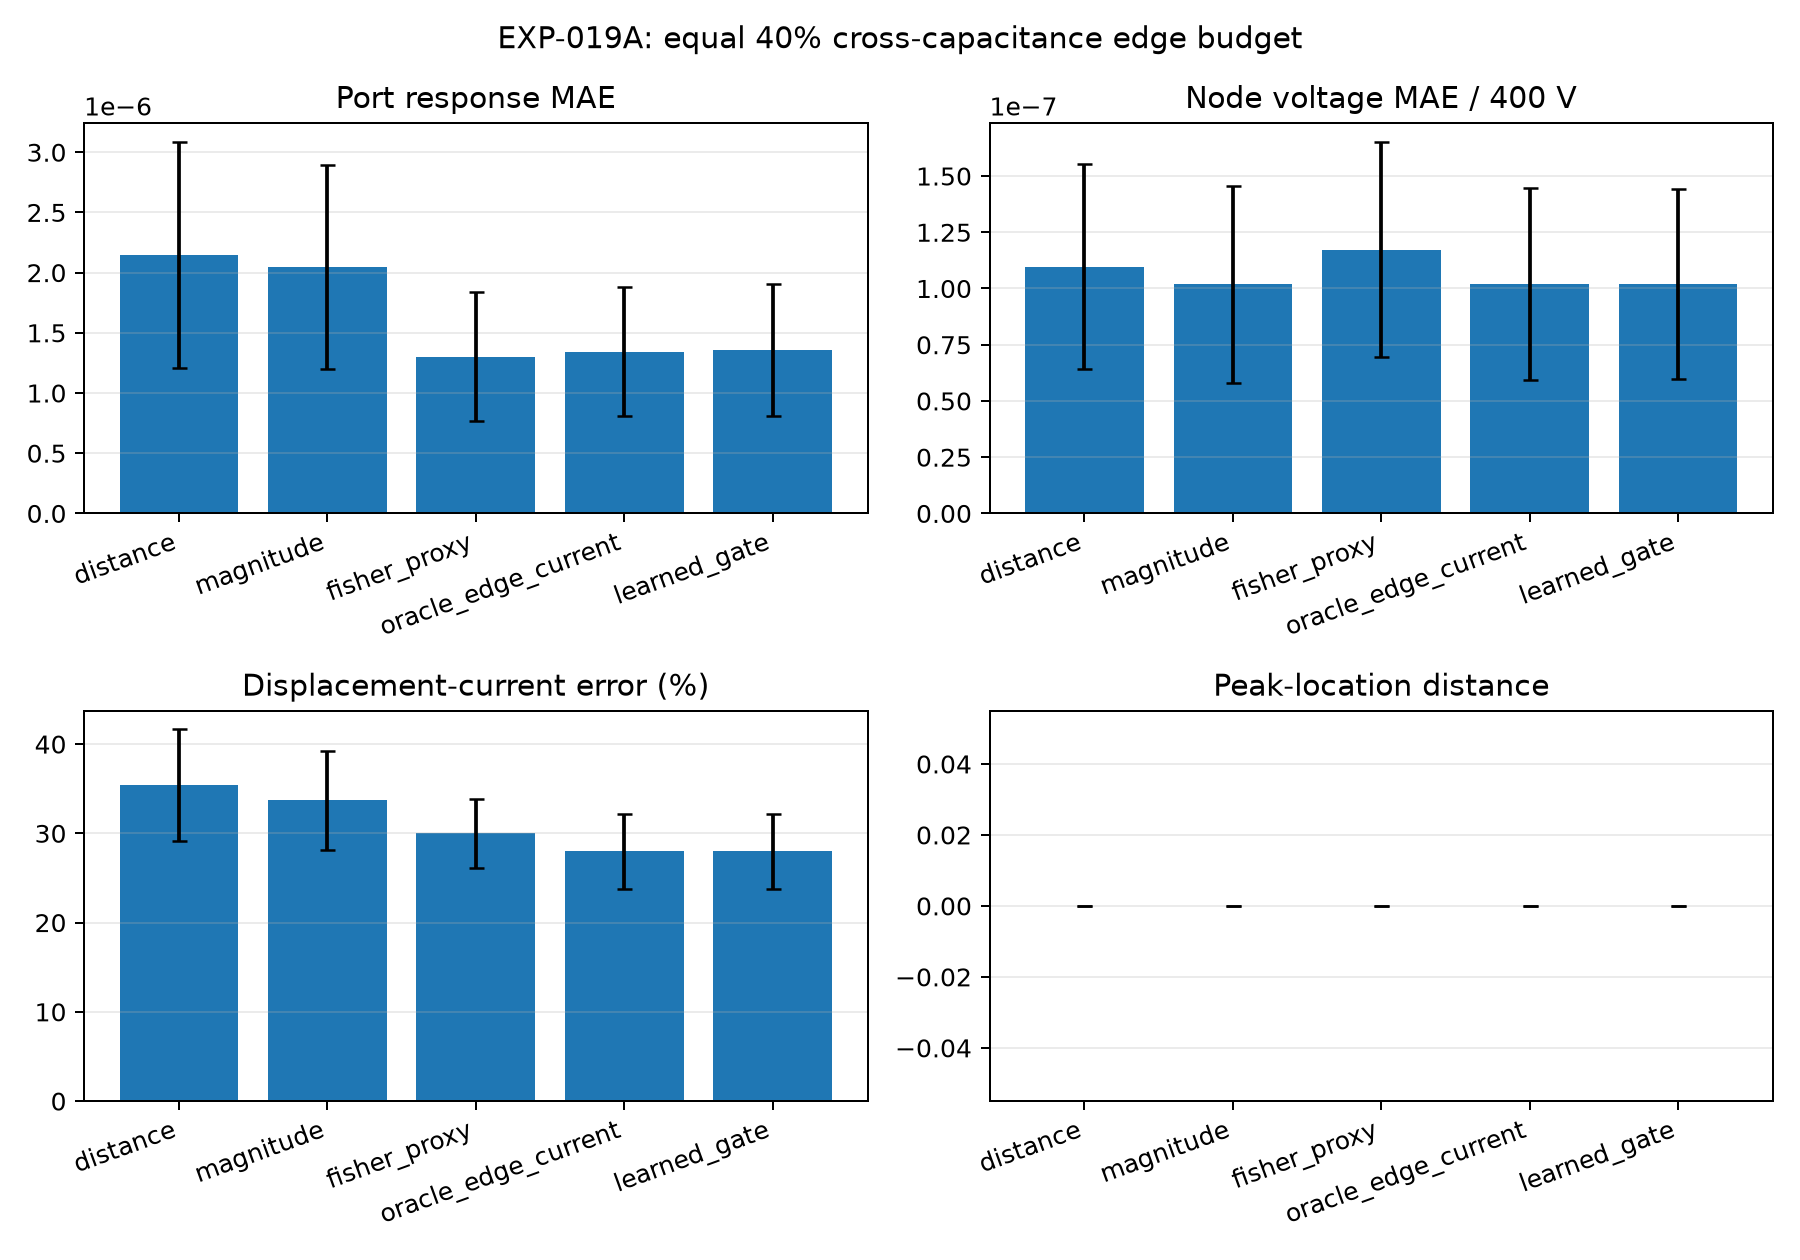
\includegraphics[width=\linewidth]{experiments/experiment19_learnable_coupling_selection_20260910/results/method_comparison.png}
\caption{40\%预算方法比较}
\end{subfigure}\hfill
\begin{subfigure}{.48\linewidth}\centering
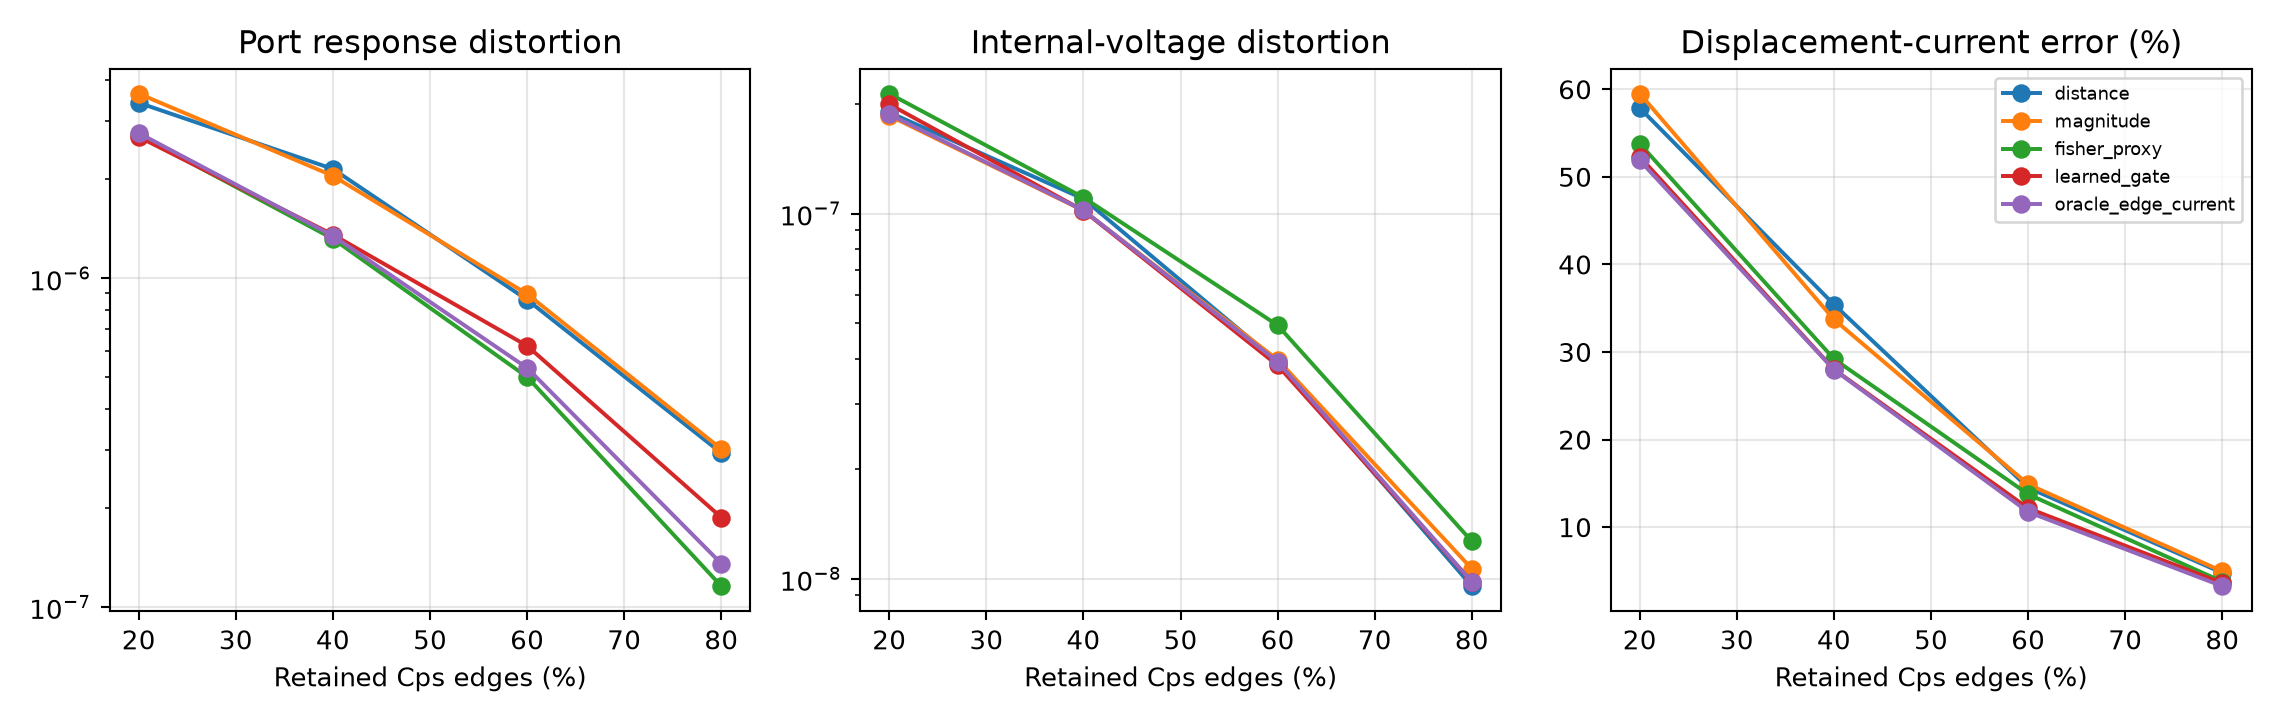
\includegraphics[width=\linewidth]{experiments/experiment19_learnable_coupling_selection_20260910/results/rate_distortion_curve.png}
\caption{边预算--失真曲线}
\end{subfigure}
\caption{只看端口误差会错误地认为激进裁剪已经足够。}
\end{figure}

\section{实验结果：COMSOL教师下的参数辨识}

\subsection{EXP21：五维参数辨识最小闭环}
EXP21 首次使用 12 个参数化 COMSOL 几何，网络输入逐匝图和多窗口复导纳，输出五个有界对数参数。结果如下：
\begin{table}[H]
\centering
\caption{EXP21 未见几何上的参数反演比较。}
\begin{tabular}{lccc}
\toprule
方法 & 五参数 MAE & 响应相对误差 & 物理迭代耗时\\
\midrule
标称模型 & -- & 7.603\% & 0\\
GNN直接反演 & 0.07569 & 5.864\% & 0\\
纯物理反演 & \textbf{0.04939} & 1.0081\% & 3.816 s\\
GNN初值+物理反演 & \textbf{0.04939} & \textbf{1.0080\%} & 3.174 s\\
\bottomrule
\end{tabular}
\end{table}
GNN 直接反演相对标称模型降低响应误差 22.87\%，但纯物理反演更准确。GNN 初值没有改善最终参数误差，只把优化时间降低约 16.8\%。因此在同模前向/反演条件下，GNN 的主要价值是快速初始化，而非精度替代。

\subsection{EXP22：模型失配下当前GNN仍未超过纯物理方法}
EXP22 加入温度和频变铜阻、非对称对地杂散电容、通道增益误差、时间偏移和测量噪声，而反演模型不知道这些变量。
\begin{table}[H]
\centering
\caption{EXP22 模型失配条件下的比较。}
\begin{tabular}{lcc}
\toprule
方法 & 五参数 MAE & 简化模型对观测响应误差\\
\midrule
标称模型 & 0.07608 & 9.506\%\\
GNN直接反演 & 0.07325 & 7.679\%\\
失配物理反演 & \textbf{0.05147} & \textbf{5.221\%}\\
GNN正则化物理反演 & 0.05478 & 5.242\%\\
\bottomrule
\end{tabular}
\end{table}
该结果否定了“只要加入 GNN 就能自动补偿未知非理想因素”的假设。温度、探头增益、对地电容和内部参数在端口上可能产生相似变化；未观测的样本特有变量不能由网络凭空恢复。

\subsection{EXP23：边选择成功，逐边动态更新只完成部分目标}
\begin{table}[H]
\centering
\caption{EXP23 静态边选择与动态更新结果。}
\begin{tabular}{lccc}
\toprule
指标 & GNN & 随机基线 & 判断\\
\midrule
电容重要边 recall@60\% & 0.853 & 0.607 & 有效\\
互感重要边 recall@60\% & 0.882 & 0.607 & 有效\\
电容变化边 F1 & 0.307 & 0.143 & 有部分定位信息\\
互感变化边 F1 & 0.107 & 0.143 & 未超过随机\\
响应误差 & 1.618\% & 标称 2.381\% & 平均降低约32\%\\
\bottomrule
\end{tabular}
\end{table}
静态重要边排序已经形成明确正结果。动态更新可改善端口重构，但不能声称逐边辨识成功，尤其互感变化定位低于随机基线。

\begin{figure}[H]
\centering
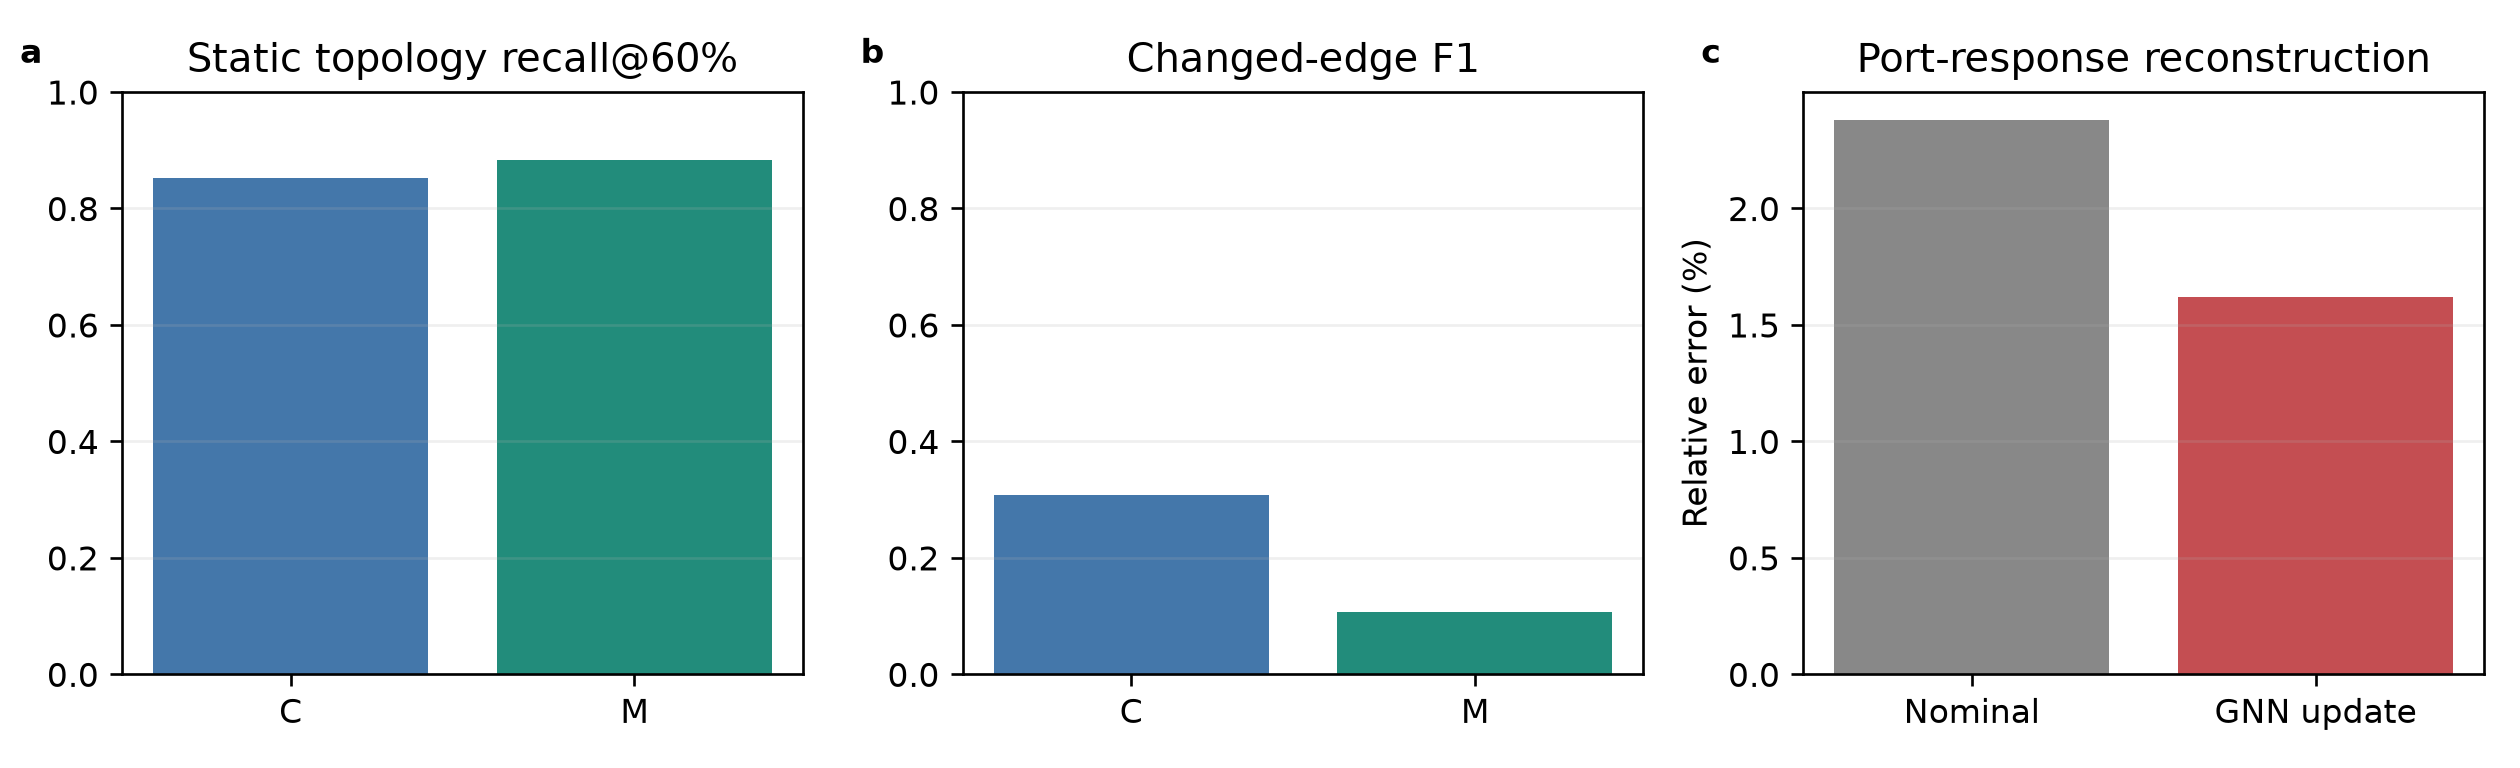
\includegraphics[width=.94\linewidth]{experiments/experiment23_edge_selection_measurement_update_20260917/figures/exp23_summary.png}
\caption{EXP23 的静态边重要性、动态变化定位与物理解码响应比较。}
\end{figure}

\begin{figure}[H]
\centering
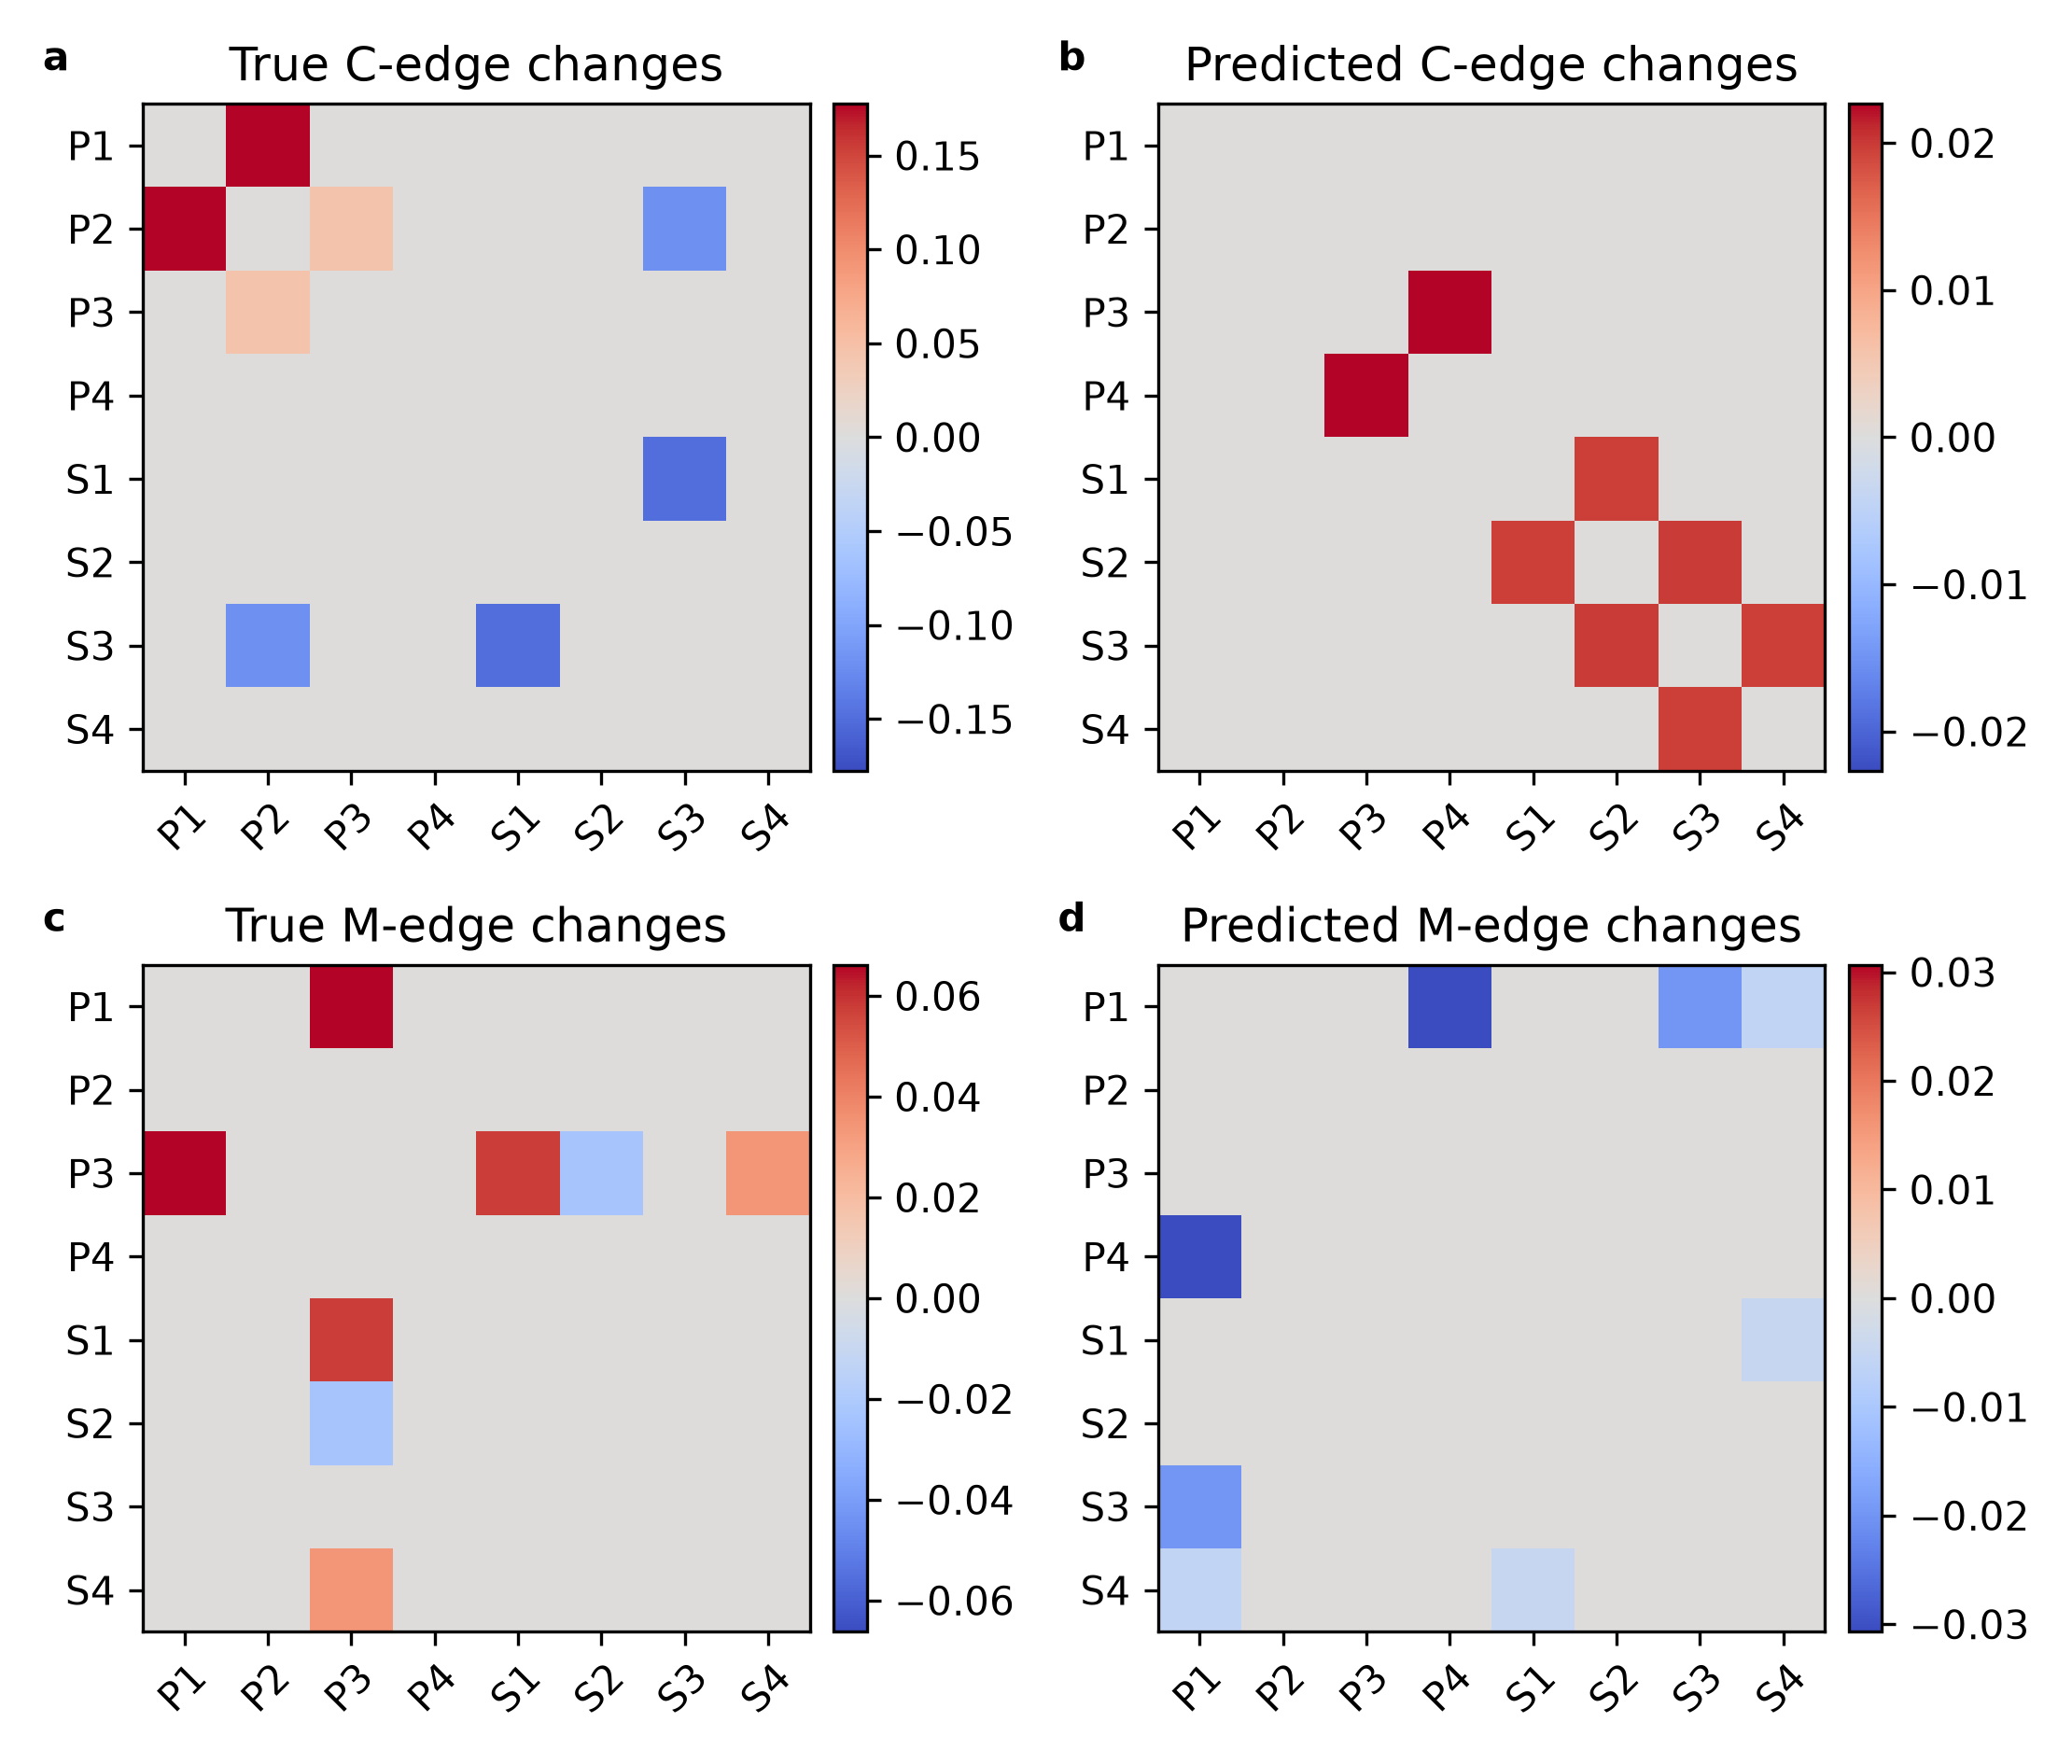
\includegraphics[width=.86\linewidth]{experiments/experiment23_edge_selection_measurement_update_20260917/figures/heldout_edge_update_example.png}
\caption{未见 COMSOL 几何上的边更新示例。图中局部拟合改善不等同于所有真实变化边均被正确恢复。}
\end{figure}

\section{为什么逐边辨识仍然困难：Fisher边界}

\subsection{56维边参数只有约3个强观测方向}
对测量特征 $\Delta\vect y$ 和边参数 $\vect z\in\R^{56}$，定义
\begin{equation}
\mat J=\frac{\partial\Delta\vect y}{\partial\vect z},
\qquad
\mat F=\mat J^{\mathsf T}\mat\Sigma^{-1}\mat J.
\end{equation}
令
\begin{equation}
\mat J=\mat U\mat\Sigma_J\mat V^{\mathsf T}.
\end{equation}
EXP24 的前三个奇异值约为 $5.33,0.672,0.110$，第四个骤降至 $1.12\times10^{-6}$。因此当前观测虽然有多个频点和复数通道，但对逐边变化只提供约三个强独立组合方向。

\begin{figure}[H]
\centering
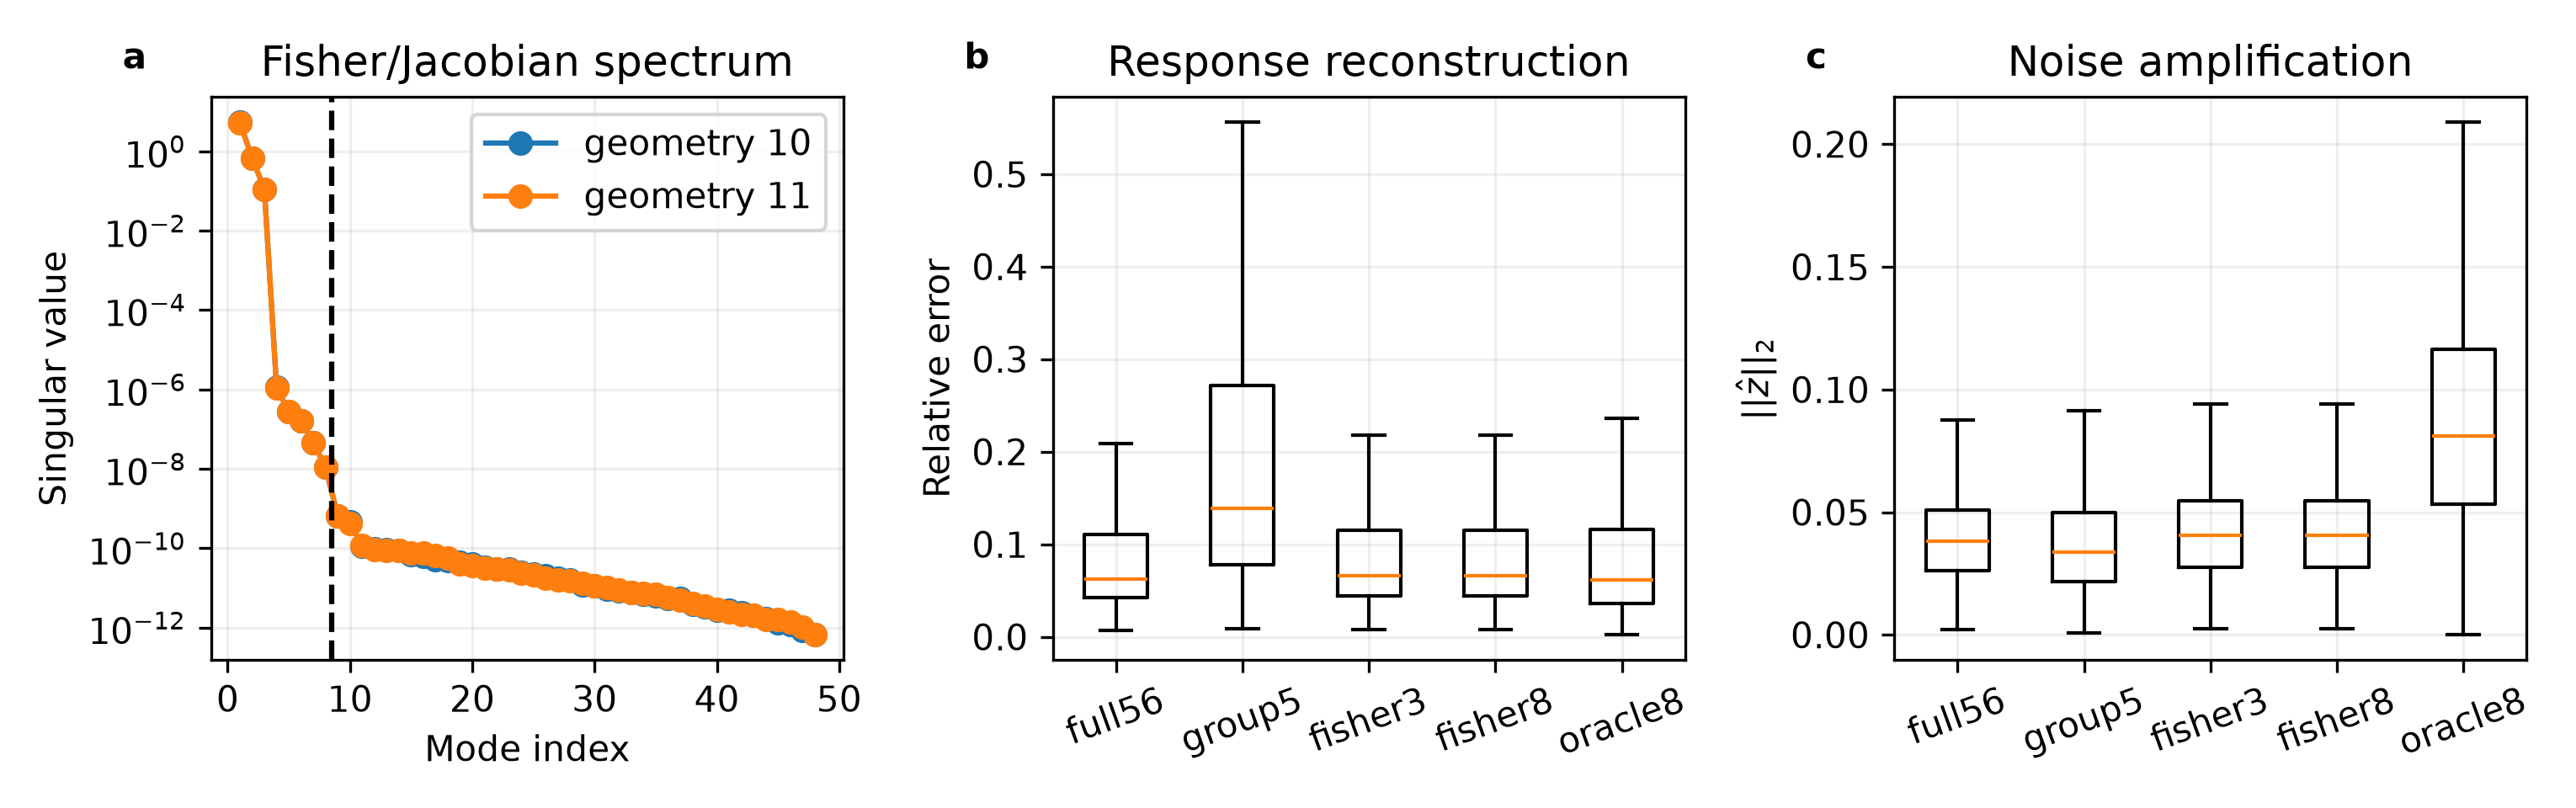
\includegraphics[width=.95\linewidth]{experiments/experiment24_fisher_identifiable_graph_modes_20260917/figures/exp24_summary.png}
\caption{EXP24 灵敏度谱及 full56、工程分组、Fisher 模态与 oracle 的比较。}
\end{figure}

在噪声标准差 0.003 下，Fisher-3 与 Fisher-8 的结果几乎相同；继续增加到第 4--8 模态没有可用信息增益。Fisher 模态能用更少变量维持与 full56 接近的响应拟合，但不能恢复真实稀疏边。

\subsection{DAB多窗口解决端口矩阵重构，不自动增加内部边秩}
EXP25 将观测链推进到 20 kHz DAB 方波、1--11 次奇次谐波、20 ns 上升时间、100 ns 死区、45 dB SNR 和 FFT 恢复。四个线性独立窗口的激励条件数中位数为 2.405，导纳测量误差为 0.0544\%；重复退化窗口和单窗口的条件数分别达到 $1.28\times10^7$ 和 $3.37\times10^{16}$，导纳误差超过 90\%。

这说明多窗口的价值是恢复完整两端口矩阵，前提是端口激励方向独立；但四个窗口并未把内部边的强可辨识维数从约 3 提高到 56。今后不得用“端口响应误差很小”单独证明内部参数辨识成功。

\section{统一指标体系及其含义}

\begin{longtable}{p{0.24\linewidth}p{0.34\linewidth}p{0.32\linewidth}}
\toprule
指标 & 数学含义 & 不能被误解为什么\\
\midrule
响应相对误差 & $\|\widehat{\mat Y}-\mat Y\|/\|\mat Y\|$ & 不能证明内部参数唯一或变化边正确\\
参数 MAE/RMSE & 对 $\vect\theta$ 或 $\vect z$ 的绝对/均方根误差 & 不同参数尺度需先归一化或使用对数坐标\\
边 recall@$k$ & 真正重要边中有多少进入 top-$k$ & 不反映被保留边参数数值是否准确\\
边 F1 & 变化边分类的精确率与召回率调和平均 & 需与随机基线和类别不平衡共同解释\\
位移电流误差 & 由物理解码后的 $I_{ps}$ 相对误差 & 比端口误差更直接检验跨绕组耦合保真\\
峰值命中率 & 预测最大内部电压位置与真值完全一致 & 当峰值位置几乎固定时可能虚高；应补 top-$k$ 和位置距离\\
无源/互易率 & 物理矩阵是否满足能量和对称约束 & 离散频点通过不等于全频带严格无源\\
Fisher奇异谱 & 灵敏度矩阵中独立观测方向的强弱 & 是局部可辨识性，不是全局唯一性证明\\
运行时间 & GNN前向、物理优化或混合方法耗时 & 必须在相同硬件和精度标准下比较\\
\bottomrule
\end{longtable}

\section{所有网络与基线的总对比}

\begin{longtable}{p{0.17\linewidth}p{0.22\linewidth}p{0.22\linewidth}p{0.29\linewidth}}
\toprule
方法 & 输入 & 输出 & 当前证据与边界\\
\midrule
FALCON homogeneous & 合并边图+工况 & 端口响应 & EXP16 MAE 0.0521；稳定基线，但忽略关系语义\\
HFT typed & 分型图+工况 & 端口响应 & EXP16 MAE 0.0538，未超过同质基线\\
Edge-centric forward & 节点+边连续属性+工况 & 端口/节点/边响应 & EXP18 端口和节点小幅优于同质模型，局部峰值定位仍弱\\
Learned edge gate & 候选 $C_{ij}$ 边+几何+工况 & 边重要性 & EXP19 接近 oracle；40\%预算仍有28\%电流误差\\
COMSOL edge-GNN inverse & COMSOL标称图+多窗口导纳 & 五维物理参数 & EXP21 直接反演改善标称，但不如纯物理优化\\
Robust edge-GNN & 标称图+失配观测 & 五维参数 & EXP22 未超过失配物理反演\\
Selector-updater GNN & 标称图+测量创新量 & 静态重要性+逐边变化 & EXP23 静态排序有效，C边定位部分有效，M边定位失败\\
Fisher-mode estimator & 灵敏度主空间+观测 & 约3个模态系数 & EXP24 给出可辨识边界；不是逐边恢复器\\
\bottomrule
\end{longtable}

\section{已经证明、尚未证明与论文级判断}

\subsection{已经有证据支持的结论}
\begin{enumerate}
  \item 逐匝 $\mat R/\mat L/\mat C$ 可统一为多关系图，并通过可微矩阵/Kron 求解器获得端口和内部响应；
  \item 显式边属性在端口和内部节点响应预测上相对同质图有小幅优势；
  \item 学习式边门控在相同预算下优于简单距离/幅值规则并接近任务 oracle；
  \item 12 个 COMSOL 几何上的五维参数反演闭环能够在 CUDA 上训练和测试；
  \item GNN 可以改善标称模型并提供物理反演初值，但当前精度仍未超过纯物理优化；
  \item 静态重要边选择已经有效，动态电容边更新存在部分可辨识信息；
  \item 当前两端口观测对 56 维边变化仅支持约 3 个强组合方向。
\end{enumerate}

\subsection{尚未完成的核心能力}
\begin{enumerate}
  \item 实机 DAB 运行数据上的跨样机参数辨识；
  \item 不依赖故障真值先验的逐边 $C/M$ 更新验证；
  \item 互感变化边可靠定位；
  \item 三维端部效应、频变损耗、磁芯非线性和真实测量链路；
  \item 多随机种子、置信区间以及跨拓扑族泛化；
  \item 证明 GNN 在精度、速度、鲁棒性或信息利用率上至少一项显著优于强物理基线。
\end{enumerate}

\subsection{当前最合适的论文主张}
目前可以写成“物理约束逐匝图辨识框架及其可辨识性边界”，但还不足以写成“实用在线逐匝全参数辨识系统”。最有说服力的贡献组合是：
\begin{enumerate}
  \item COMSOL/正常模型构建多关系逐匝图；
  \item GNN 学习任务相关的静态耦合结构；
  \item Fisher/SVD 将动态更新压缩到可辨识模态；
  \item DAB 多窗口测量条件化 GNN 估计模态系数；
  \item 精确物理解码器恢复内部状态并强制物理合法；
  \item 实机或高保真独立模型验证仿真到现实迁移。
\end{enumerate}

\section{推荐的最终网络结构}

\subsection{结构编码器}
静态图编码器接收节点几何、绕组身份、边类别、标称 $C_{ij}/M_{ij}$ 和距离特征，产生节点/边嵌入：
\begin{equation}
(\mat H,\mat E)=E_{graph}(\mathcal G_0).
\end{equation}
边选择头输出任务相关重要性 $s_{ij}^{C},s_{ij}^{M}$。这里的目标不是无限删边，而是形成结构化候选集和边组。

\subsection{测量编码器}
对 DAB 多窗口复频谱及其测量质量进行编码：
\begin{equation}
\vect q=E_{meas}\left(\{V_1,I_1,V_2,I_2,f,w,\gamma^2,\mathrm{SNR}\}\right).
\end{equation}
测量编码器需同时输入窗口激励矩阵的最小奇异值或条件数，防止退化窗口被错误解释为参数不变。

\subsection{Fisher模态输出而非自由逐边输出}
令 $\mat B\in\R^{56\times r}$ 为 Fisher 主模态或物理区域基，当前证据建议首版 $r\approx3$：
\begin{equation}
\widehat{\vect\eta}=H_{mode}(\mat H,\mat E,\vect q),
\qquad
\Delta\widehat{\vect z}=\mat B\widehat{\vect\eta}.
\end{equation}
网络也可输出异方差不确定度 $\widehat{\mat\Sigma}_\eta$，在信息不足时拒绝更新。

\subsection{物理解码与训练目标}
\begin{equation}
\widehat{\mat C},\widehat{\mat L}=\mathrm{Stamp}(\mat C_0,\mat L_0,\Delta\widehat{\vect z}),
\end{equation}
\begin{equation}
\widehat{\mat Y},\widehat{\vect v}_{int},\widehat{\vect i}_{ps}
=\mathrm{PhysicsSolver}(\widehat{\mat C},\widehat{\mat L},\mat R,\vect u).
\end{equation}
建议损失为
\begin{align}
\mathcal L={}&\lambda_Y\mathcal L_Y+lambda_I\mathcal L_I
+\lambda_\eta\mathcal L_\eta+lambda_{edge}\mathcal L_{edge}\\
&+\lambda_{pass}\mathcal L_{passive}
+\lambda_{rec}\mathcal L_{reciprocal}
+\lambda_{unc}\mathcal L_{NLL}.
\end{align}
其中 $\mathcal L_Y$ 约束可测端口，$\mathcal L_I$ 约束跨绕组位移电流或共模观测，$\mathcal L_\eta$ 仅在仿真标签可用时监督模态参数，物理项保证输出可部署。

\section{下一阶段实验设计}

\subsection{最小必要补强}
\begin{enumerate}
  \item 将 EXP23 的自由逐边更新头替换为 EXP24 的 Fisher-3 模态头；
  \item 比较 MLP、homogeneous、typed、edge-centric 四种测量编码器，保持相同输出模态和物理解码器；
  \item 每个方法至少运行 5 个随机种子，报告均值和 95\% 置信区间；
  \item 增加 zero-update、纯物理、GNN直接、GNN+物理四个强基线；
  \item 在两端口之外逐项加入共模电流、参考导体电流或第三端口观测，测量可辨识秩的增量；
  \item 用独立 COMSOL 几何或更高保真模型作为测试教师，避免前向/反演同模；
  \item 最终再进入低压样机，先做正常模型标定和已知附加电容/局部位置扰动。
\end{enumerate}

\subsection{验收标准}
主方法至少应满足：
\begin{itemize}
  \item 在未见几何和未见工况上，相对纯物理反演显著降低模态参数误差或达到相同误差但显著加速；
  \item 物理解码的无源、互易和正定合规率为 100\%；
  \item 相比 zero-update，在内部任务上有稳定增益，而不仅是端口曲线更接近；
  \item 对退化窗口能够输出高不确定度或拒绝更新；
  \item 新增观测后 Fisher 强模态数或最小奇异值出现可解释提升。
\end{itemize}

\section{结论}
项目已经从“GNN 使用已知边预测响应”推进到“GNN 选择重要边并依据测量更新耦合参数”的初步闭环。FALCON 风格同质图提供了必要 baseline，HFT typed 和 edge-centric 结构验证了物理关系表示的价值，可学习门控证明了任务相关边排序可被学习，COMSOL 教师使参数辨识从手工合成数据迈向场仿真数据，EXP23 则首次实现静态边选择和动态边更新。然而，EXP22--25 同时说明，当前主要瓶颈不是网络容量，而是观测信息维数和未建模变量混淆。最合理的下一步是把 GNN 输出从 56 维自由边更新收缩为约 3 个 Fisher 可辨识图模态，并通过额外共模/参考导体观测逐步增加可辨识秩。只有在强物理基线、多随机种子、独立高保真测试和最终样机数据上保持优势，才适合宣称工程级在线逐匝参数辨识。

\appendix
\section{关键实验数字速查}
\begin{longtable}{p{0.12\linewidth}p{0.36\linewidth}p{0.42\linewidth}}
\toprule
实验 & 关键数字 & 正确结论\\
\midrule
EXP16 & GNN MAE 0.0521/0.0538；参数缩放误差 7.16\% & FALCON基线可运行，响应拟合不等于参数唯一\\
EXP18 & edge-centric residual：端口 0.02707、节点 0.004263、边电流 0.01230 & 显式边属性有小幅价值，局部定位仍弱\\
EXP19 & 40\%预算 learned 28.01\%，oracle 27.98\%；80\%预算约3.60\% & 网络会排序，但真实任务需要保留较多边\\
EXP21 & GNN响应5.864\%，物理1.0081\%，混合1.0080\% & GNN主要提供初值和16.8\%时间改善\\
EXP22 & GNN参数0.07325，物理0.05147，混合0.05478 & 当前GNN未解决模型失配\\
EXP23 & C/M静态recall 0.853/0.882；C/M动态F1 0.307/0.107 & 静态边选择有效，互感逐边更新失败\\
EXP24 & 奇异值 $5.33,0.672,0.110,1.12\times10^{-6}$ & 56维边变化只有约3个强方向\\
EXP25 & 独立窗口导纳误差0.0544\%；单窗口93.66\% & 多窗口恢复端口矩阵，但不自动增加内部边秩\\
\bottomrule
\end{longtable}

\section{代码入口}
\begin{longtable}{p{0.22\linewidth}p{0.68\linewidth}}
\toprule
功能 & 仓库入口\\
\midrule
物理图与求解器 & \code{experiments/experiment15\_hft\_graph\_physics\_20260901/}\\
FALCON/HFT GNN & \code{experiments/experiment16\_falcon\_hft\_gnn\_20260909/}\\
异构正向GNN & \code{experiments/experiment18\_local\_hetero\_gnn\_20260910/}\\
学习边门控 & \code{experiments/experiment19\_learnable\_coupling\_selection\_20260910/}\\
COMSOL五维反演 & \code{experiments/experiment21\_comsol\_gnn\_minimal\_20260916/}\\
模型失配反演 & \code{experiments/experiment22\_model\_mismatch\_robust\_inverse\_20260916/}\\
边选择与更新 & \code{experiments/experiment23\_edge\_selection\_measurement\_update\_20260917/}\\
Fisher图模态 & \code{experiments/experiment24\_fisher\_identifiable\_graph\_modes\_20260917/}\\
DAB PWM观测 & \code{experiments/experiment25\_dab\_pwm\_time\_domain\_observability\_20260917/}\\
\bottomrule
\end{longtable}

\end{document}
